\documentclass[12pt,a4paper]{article}
\usepackage[utf8]{inputenc}
\usepackage[margin=2cm]{geometry}
\usepackage{amsmath}
\usepackage{amssymb}
\usepackage{amsthm} 
\usepackage{graphicx}
\usepackage{mathtools}
\usepackage{algorithm}
\usepackage{algorithmic}
\usepackage[normalem]{ulem}
\DeclarePairedDelimiter{\abs}{\lvert}{\rvert}
\newcommand{\inter}{\begin{matrix}\prod\end{matrix}}
\DeclarePairedDelimiter{\norma}{\lVert}{\rVert}
 
\begin{document}

\section[Lezione 21 - Metodo di Gauss, calcolo determinante]{Lezione 21 - Riduzione a forma triangolare col metodo di eliminazione gaussiana (meg), calcolo del determinante}
In questa lezione ripasseremo il METODO DI ELIMINAZIONE GAUSSIANA (MEG) per la riduzione di una matrice quadrata non singolare a forma \uline{triangolare}.\\ Il $meg$ è già stato introdotto nel corso di algebra lineare e geometria, qui ne richiameremo i tratti fondamentali con una particolare attenzione a come implementarlo in modo stabile in aritmetica floating-point.\\Come prima applicazione ci concentreremo sul calcolo del determinante di una matrice quadrata, riservando le prossime 2 lezioni all'analisi del $meg$ per la soluzione di sistemi lineari.\\Sia $A\in\mathbb{R}^{n\times n}$: ricordiamo che il \uline{determinante} di $A$, che qui indicheremo con $det(A)$, è una quantità fondamentale per capire le proprietà di una matrice quadrata, infatti 
\begin{center}
    $det(A)\neq0\iff Ax=b$ ha soluzione unica $\forall b$ $\iff$ $A$ è invertibile 
\end{center}
Una delle definizioni di $det(A)$ si può dare in modo ricorsivo con la formula di Laplace, che permette di definire il $det$ di una matrice $n\times n$ utilizzando determinanti di matrici $(n-1)\times(n-1)$.

\subsection{Formula di Laplace}
\begin{center}
    $det(A)=A$ se $A\in\mathbb{R}$
\end{center}
\begin{equation*}
    det(A)=\sum_{j=1}^n(-1)^{i+j}det(A_{ij})
\end{equation*}
(sviluppo secondo la riga $i$) dove $A_{ij}$ è la sottomatrice $(n-1)\times(n-1)$ ottenuta da $A$ cancellando riga $i$ e colonna $j$, ad esempio per $n=3$ e $i=1$
\begin{center}
    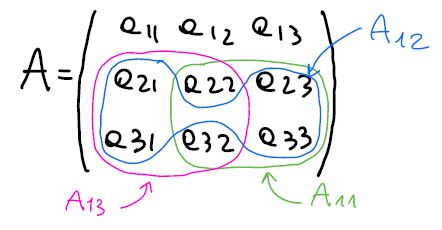
\includegraphics[scale=0.5]{pag4.jpg}    
\end{center}
Da questa definizione,
\begin{equation*}
    A\in\mathbb{R}^{2\times 2}\Rightarrow det(A)=a_{11}a_{22}-a_{12}a_{21}
\end{equation*}
\begin{equation*}
        A\in\mathbb{R}^{3\times 3}\Rightarrow det(A)=a_{11}det(A_{11})-a_{12}det(A_{12})+a_{13}det(A_{13})
\end{equation*}
\begin{equation*}
    = a_{11}(a_{22}a_{33}-a_{23}a_{32})-a_{12}(a_{21}a_{33}-a_{23}a_{31})+a_{13}(a_{21}a_{32}-a_{22}a_{31})
\end{equation*}
La formula di Laplace è molto importante per studiare le proprietà del determinante ed è abitualmente usata per calcolare a mano determinanti di matrici $2\times 2$ e $3\times 3$.\\
Ma già mettendosi a calcolare un determinante nel caso $4\times 4$ si comincia a fare fatica e nel caso $5\times5$ ci si accorge che la quantità di risultati intermedi da tenere e di calcolare comincia a crescere molto rapidamente.\\In realtà la difficoltà diventa molto presto insormontabile anche implementando la formula al calcolatore, come si vede nella tabella qui sotto, dove i tempi di calcolo corrispondono ad usare un computer da $1Gflops$ ($10^9$ operazioni aritmetiche al secondo, che è la velocità attuale di un PC) e da $1Pflops$ ($10^{15}$ operazioni aritmetiche al secondo, un supercomputer).

\subsubsection{TABELLA 1 (det con Laplace)}
\[ \begin{split}
	& \uline{n\quad\quad 1Gflops\quad\quad 1Pflops}\\
	&  10\quad\quad 10^{-3}sec\quad\quad 10^{-9}sec\\
	&  15\quad\quad 40min\quad\quad 2\cdot10^{-3}sec\\
	& 20\quad\quad 10^{2}anni\quad\quad 80min\\
	& 25\quad\quad 10^{9}anni\quad 10^{3}anni\\
	& 100\quad 10^{141}anni\quad\quad 10^{135}anni\\ 
\end{split} \]
E' evidente che la formula di Laplace è inapplicabile già per il calcolo di determinanti con $n$ relativamente piccolo, visto che per $n=20$ un PC impiegherebbe 1 miliardo di anni e quindi un supercomputer ben 1 milione di volte più veloce ``solo" 100 anni.\\Perchè i tempi esplodono in questo modo?\\Per stimare il costo computazionale, possiamo contare in modo semplice il \# di moltiplicazioni, che chiamiamo $c_n^{molt}$.\\
E' chiaro che dovendo calcolare $n$ determinanti $(n-1)\times (n-1)$ (il prodotto per $(-1)^{i+j}$ è solo un cambio di segno per $i+j$ dispari) si ha che 
\begin{equation*}
    c_n^{molt} = n c_{n-1}^{molt}
\end{equation*}
e chiaramente
\begin{equation*}
    c_2^{molt} = 2
\end{equation*}
Quindi
\begin{equation*}
    \begin{split}
        & c_3^{molt} = 3 \cdot c_2^{molt} = 3\cdot 2 \\
        & c_4^{molt} = 4 \cdot c_3^{molt} = 4\cdot 3\cdot 2 \\
        & \vdots \\
        & c_n^{molt} = n(n-1)\cdot ... \cdot 4\cdot 3\cdot 2 = n!
    \end{split}
\end{equation*}
Ne consegue che il costo computazionale della formula di Laplace (in cui ci sono anche somme algebriche) è $c_n^{lapl} > n!$ (si può far vedere -non richiesto- che $c_n^{lapl} \sim 2n!$, $n \to \infty$). \\
Questo spiega perfettamente l'esplosione dei tempi di calcolo vista la rapidissima crescita del fattoriale
\begin{equation*}
    \bigl( \frac{n}{2} \bigr)^ {\frac{n}{2}} < n! < n^n
\end{equation*}
ad es. $10! \approx 3.7 \cdot 10^6$, $15! \approx 1.3 \cdot 10^{12}$, $20! \approx 2.4 \cdot 10^{18}$, $25! \approx 1.6 \cdot 10^{25}$.\\
E' chiaro che vogliamo poter calcolare determinanti $20 \times 20$, $25 \times 25$, $100 \times 100$ e anche ben oltre in tempi ragionevoli, quindi è necessario un algoritmo alternativo il cui costo cresca possibilmente come una potenza di $n$ con esponente piccolo. \\
E' qui che entra in gioco l'oggetto della lezione, il meg.

\subsection{Metodo di eliminazione gaussiana}
Il meg è basato su 2 proprietà fondamentali del determinante che riguardano trasformazioni (per righe o per colonne, qui lavoreremo per righe) della matrice. \\
Queste proprietà sono:
\begin{enumerate}
    \item sostituendo alla riga $k$ la somma della riga $k$ con la riga $i$ moltiplicata per uno scalare, in simboli
    \begin{equation*}
        R_k \underset{\text{assegnazione}}{:=} \underset{\text{riga $k$-esima}}{R_k} + \alpha \underset{\text{riga $i$-esima}}{R_i}, \ \alpha \in \mathbb{R}
    \end{equation*}
    il determinante non cambia
    \item scambiando due righe il determinante cambia segno
\end{enumerate}
Entrambe possono essere dimostrate (non richiesto) per induzione tramite la formula di Laplace.\\
Queste 2 trasformazioni elementari sono alla base del meg (per righe), che permette di ridurre una matrice quadrata non singolare in forma triangolare.\\
Richiamiamo come opera il meg con un semplice esempio $3 \times 3$
\begin{equation*}
    A=\begin{pmatrix}
       1 & 2 & 1 \\
       2 & 2 & 3 \\
       -1 & -3 & 0
    \end{pmatrix}
\end{equation*}
L'idea come noto è di usare ripetutamente la 1) per mettere zeri in ogni colonna sotto la diagonale principale, in modo da arrivare a 
\begin{equation*}
    U = \begin{pmatrix}
        u_{11} & u_{12} & u_{13} \\
        0 & u_{22} & u_{23} \\
        0 & 0 & u_{33}
    \end{pmatrix}
\end{equation*}
TRIANGOLARE SUPERIORE, che ha lo stesso determinante (a meno di scambi di righe cioè a meno del segno se il numero di scambi è dispari).\\
Si vede subito (basta di nuovo usare la formula di Laplace sviluppata sull'ultima riga) che
\begin{center}
    $det(U) = \inter u_{ii} = u_{11} u_{22} u_{33}$
\end{center}
\begin{equation*}
    \begin{split}
        & \underset{=A^{(1)}}{A}=\begin{pmatrix}
              1 & 2 & 1 \\
              2 & 2 & 3 \\
              -1 & -3 & 0
        \end{pmatrix} \overset{R_2 := R_2 + (-2) R_1}{\longrightarrow} \begin{pmatrix}
                  1 & 2 & 1 \\
                  0 & -2 & 1 \\
                 -1 & -3 & 0
        \end{pmatrix} \\
        & \overset{R_3 := R_3 + R_1}{\longrightarrow} A^{(2)} \begin{pmatrix}
                  1 & 2 & 1 \\
                  0 & -2 & 1 \\
                  0 & -1 & 1
        \end{pmatrix} \overset{R_3 := R_3 + ( -\frac{1}{2}) R_2}{\longrightarrow} A^{(3)} = U \begin{pmatrix}
                  1 & 2 & 1 \\
                  0 & -2 & 1 \\
                  0 & 0 & \frac{1}{2}
        \end{pmatrix}
    \end{split}
\end{equation*}
da cui (non essendoci stati scambi di righe)
\begin{equation*}
    det(A) = det(U) = -1
\end{equation*}
Da questo semplice esempio si vede che il meg consiste in una sequenza di $n-1$ trasformazioni
\[
A^{(1)} = A \rightarrow A^{(2)} \rightarrow A^{(3)} \rightarrow \dotso \rightarrow A^{(n)} = U
\]
dove la $U$ finale è triangolare superiore (cioè gli elementi sotto la diagonale sono tutti nulli) e al passo i-esimo la struttura schematica di $A^{(i)}, \ 1 \le i \le n-1$ è
\begin{center}
    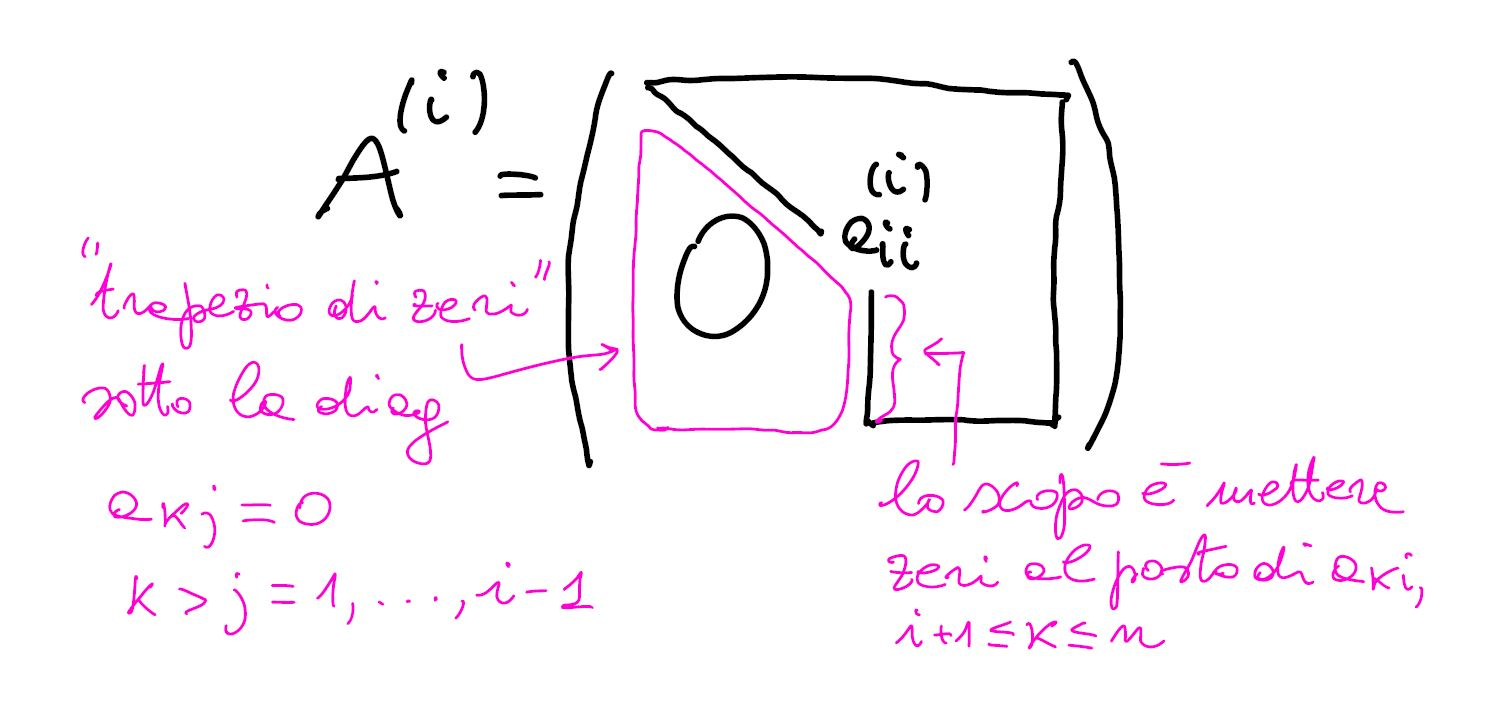
\includegraphics[width = 0.7\textwidth]{pag16.jpg}
\end{center}
Se $a_{ii}^{(i)} \neq 0$ (cioè se l'elemento diagonale di $A^{(i)}$ è non nullo) si può propagare a destra la struttura del trapezio di zeri con le trasformazioni
\[
\mathcal{R}_k^{(i+1)} := \mathcal{R}_k^{(i)} + (-\frac{a_{ki}^{(i)}}{a_{ii}^{(i)}}) \cdot \mathcal{R}_i^{(i)}, \ i+1 \le k \le n
\]
che mettono lo zero al posto $k,i$ visto che
\[
a_{ki}^{(i+1)} = a_{ki}^{(i)} + (-\frac{a_{ki}^{(i)}}{a_{ii}^{(i)}}) \cdot a_{ii}^{(i)} = 0
\]
Se invece $a_{ii}^{(i)} = 0$ si va a cercare un elemento $a_{ki} \neq 0, \ k > i$ e si scambia la riga $k$ con la riga $i$, in modo di non avere zero sulla diagonale (in questo caso il determinante cambia segno).\\
Questo è sempre possibile se $A$ è non singolare: infatti se
\[ a_{ii}^{(i)} = 0, \ a_{ki}^{(i)} = 0,\ k > i, \ det(A^{(i)}) = 0 \]
come si può controllare con la formula di Laplace (per induzione, sviluppando secondo l'ultima riga) e quindi
\[ det(A) = \pm det(A^{(i)}) = 0 \]
Fra l'altro, questo significa anche che se la matrice $A$ è singolare l'algoritmo prima o poi si accorge che il determinante è nullo trovando zero sulla diagonale e su tutti gli elementi sotto la diagonale nella stessa colonna (altrimenti arriverebbe alla fine trovando un determinante non nullo).\\
Osserviamo che in questa procedura di gestione della situazione critica in cui $a_{ii}^{(i)} = 0$ è essenziale scambiare con una riga $k > i$ (altrimenti la struttura di zeri a trapezio nella parte sinistra verrebbe alterata).\\
Il passo i-esimo per matrici non singolari (a meno del possibile scambio di righe) è
\begin{center}
    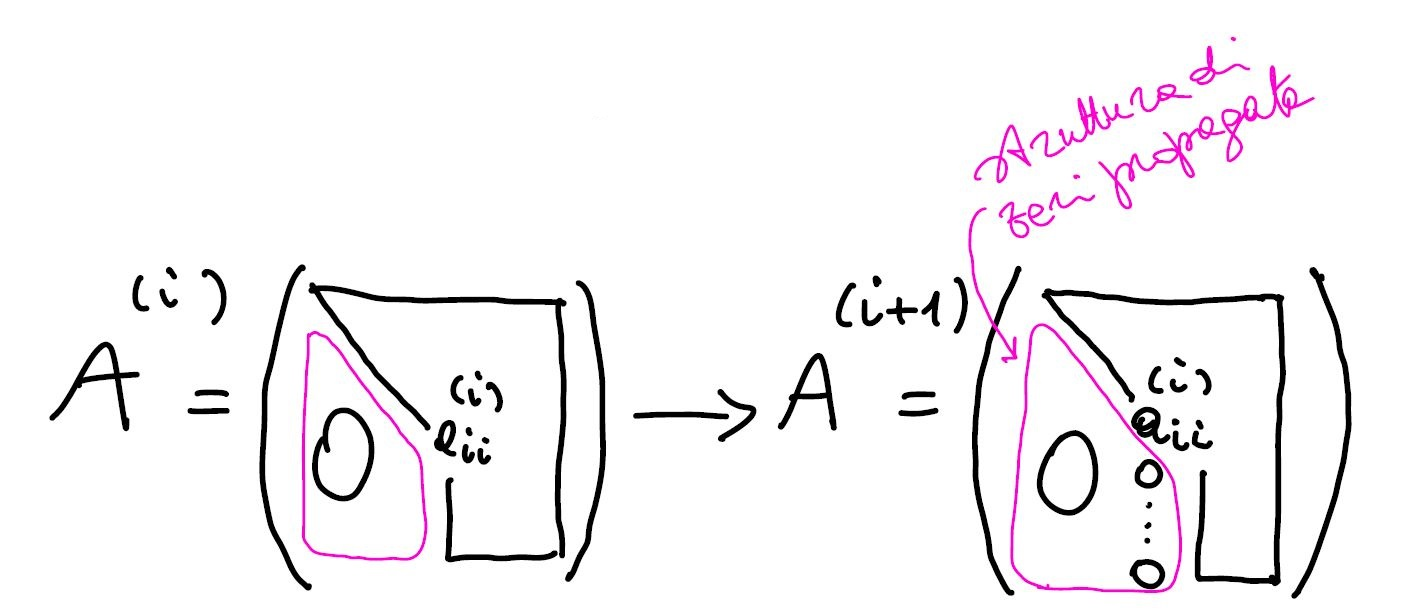
\includegraphics[width = 0.65\textwidth]{pag20.jpg}
\end{center}
cioè la struttura a trapezio di zeri viene propagata verso destra fino ad arrivare ad un triangolo di zeri al passo $n-1$ con $A^{(n)} = U$.\\
Conviene a questo punto sintetizzare il meg con uno PSEUDO-CODICE in cui la necessità di avere $a_{ii}^{(i)} \neq 0$ viene implementata in modo automatico con un'operazione detta di PIVOTING (per righe) di cui discuteremo il significato in aritmetica floating-point.\\
Il PIVOTING consiste nel cercare al passo i-esimo l'elemento $a_{ki}^{(i)}, \ k \ge i$ di massimo modulo e scambiarne la riga con la i-esima.

\subsection{Algoritmo di calcolo del MEG}
\begin{algorithm}
\caption{PSEUDO-CODICE DEL MEG}
\begin{algorithmic}
    \REQUIRE $n \in \mathbb{N}, \ A \in \mathbb{R}^{n \times n}, \ \varepsilon > 0$ (tolleranza)
    \ENSURE $B = U$ e \verb|determ| = $det(A)$
    \STATE \verb|// inizializzazione|
    \STATE $B \leftarrow A;$ \verb|// B matrice ausiliaria|
    \STATE $s \leftarrow 0;$ \verb|// contatore del numero di scambi|
    \FOR{$i=1, \ \dotso, \ n-1$}
        \STATE \verb|// pivoting|
        \STATE ``cerca $p \ge i: \ \abs{b_{pi}} \ge \abs{b_{ki}}, \ i \le k \le n$"
        \IF{$\abs{b_{pi}} < \varepsilon$}
            \STATE ``esci con warning: matrice (quasi) singolare"
        \ENDIF
        \IF{$p>i$}
            \STATE ``scambia $\mathcal{R}_p$ con $\mathcal{R}_i$"
            \STATE \verb|s++;|
        \ENDIF
        \STATE \verb|// azzeramenti in colonna i sotto la diagonale|
        \FOR{$k=i+1, \ \dotso, \ n$}
            \STATE $\mathcal{R}_k \leftarrow \mathcal{R}_k + (-b_{ki}/b_{ii}) \cdot \mathcal{R}_i$
        \ENDFOR
    \ENDFOR
    \STATE \verb|determ = | $(-1)^s \cdot \prod_{i=1}^n b_{ii}$
\end{algorithmic}
\end{algorithm}
\uline{Output}: $B=U$ e determ=$det(A)$\\
Facciamo qualche osservazione sull'implementazione del meg riassunta dallo pseudo-codice.\\
Innanzitutto il significato dell'assegnazione iniziale $B \leftarrow A$: lo scopo è quello di calcolare il determinante trasformando una \uline{copia} della matrice, in modo da non modificare la matrice di partenza che l'utente potrebbe voler mantenere inalterata per altri usi (ed è esattamente quello che succede ad es. in Matlab scrivendo \verb|det(A)|).\\
D'altra parte la matrice $B$ in output altro non è che la matrice triangolare superiore $U$ risultato dell'eliminazione gaussiana.\\
Poi un paio di osservazioni sull'operazione di pivoting (il nome viene da ``pivot", l'elemento più grande, basta pensare all'uso del termine nel basket).\\
\begin{enumerate}
\item Il primo scopo del pivoting è di mettere qualcosa di diverso da zero sulla diagonale se al passo i-esimo risulta $b_{ii}=0$, senza alterare la struttura di zeri a sinistra e quindi cercando sotto la diagonale per l'eventuale scambio.\\Sappiamo che se $b_{ii}=0$ e $b_{ki}=0\quad \forall k\geq i$ allora $det(B)=0$.\\Però del punto di vista numerico in aritmetica floating-point non ha molto senso un controllo di uguaglianza esattamente a zero ma ha più senso un controllo del tipo $\underset{k\geq i}{max}|b_{ki}|\leq \varepsilon$ con $\varepsilon$ molto piccolo, ad esempio $\varepsilon=10^{-20}$, perchè allora ci si aspetta che $det(B)$ sia estremamente piccolo e quindi che la matrice $A$ sia ``quasi singolare".
\item Ma c'è un altro motivo per il pivoting (e anche per non accettare pivot troppo piccoli), che è un motivo di stabilità numerica dell'algoritmo. Infatti, utilizzare elementi diagonali piccoli, che compaiono poi a denominatore nel coeff. $-\frac{b_{ki}}{b_{ii}}$ del procedimento di eliminazione, implica la creazione di numeri grandi e arrotondati che un pò alla volta portano ad una forte perdita di precisione nelle inevitabili sottrazioni presenti nel metodo (più grandi sono $x$ e $y$ nella sottrazione $x-y$, meno vicini devono essere in termini assoluti per rendere grandi i coeff. di amplificazione $w_1=\frac{|x|}{|x-y}$ e $w_2=\frac{|y|}{|x-y|}$).\\Quindi il pivoting ha un effetto di STABILIZZAZIONE del $meg$.\\\\
\end{enumerate}

\subsubsection{Costo computazionale del MEG}
Per concludere la lezione vale la pena calcolare il costo computazionale del $meg$.\\Questo è semplice analizzando lo pseudo-codice: infatti tralasciando i confronti e scambi del pivoting e concentrandosi sul \# di flops, che chiamiamo $c_n^{meg}$, quello che conta sono i due cicli ``for" innestati.\\Ora, l'operazione vettoriale tra righe nel ciclo interno ha un costo di $n$ moltiplicazioni e $n$ somme (poi c'è una singola divisione che asintoticamente non contribuisce alla parte principale).\\Quindi possiamo scrivere
\begin{equation*}
    c_n^{meg}\sim\sum_{i=1}^{n-1}\sum_{k=i+1}^{n}2n=2n\sum_{i=1}^{n-1}(n-i)\underset{j=n-i}{=}2n\sum_{j=1}^{n-1}j=2n\cdot\frac{n(n-1)}{2}=n^3-2n^2\sim n^3,\  \  \  \  n\rightarrow\infty
\end{equation*}
dove tra il 3o e 4o passaggio la sommatoria è stata tolta perchè somma dei primi $n-1$ numeri naturali. Si vede che il $meg$ ha costo computazionale che cresce come il cubo di $n$ per $n$ grande.\\In realtà non ha molto senso fare le operazioni vettoriali sugli interi vettori riga, perchè all'iterazione i-esima i primi $i-1$ elementi delle righe $\mathcal{R}_i$ e $\mathcal{R}_k$ sono nulli e restano nulli nella combinazione lineare. D'altra parte anche l'operazione di annullamento dell'elemento $k,i$
\begin{equation*}
    b_{ki}:=b_{ki}+(-\frac{b_{ki}}{b_{ii}})\ast b_{ii}
\end{equation*}
non va fatta visto che il risultato è zero ma in aritmetica floating point potrebbe non esserlo per effetto degli arrotondamenti, quindi conviene assegnare direttamente il valore 0.\\L'operazione vettoriale va fatta allora solo sul segmento di vettore con indici da $i+1$ a $n$, cioè in notazione simil-Matlab
\begin{equation*}
    \mathcal{R}_k[i+1:n]:=\mathcal{R}_k[i+1:n]+(-\frac{b_{ki}}{b_{ii}})\ast \mathcal{R}_i[i+1:n]
\end{equation*}
con un costo di $2(n-i)+1$ flops.\\Allora
\begin{equation*}
    c_n^{meg}\sim\sum_{i=1}^{n-1}\sum_{k=i+1}^{n}2(n-i)=2\sum_{i=1}^{n-1}(n-i)^2\underset{j=n-i}{=}2\sum_{j=1}^{n-1}j^2\sim \frac{2}{3}n^3
\end{equation*}
ottenendo il costo asintotico effettivo del $meg$ visto che
\begin{equation*}
    \frac{(n-1)^3}{3}<\sum_{j=1}^{n-1}j^2<\frac{n^3}{3}-1
\end{equation*}
(la dimostrazione non è richiesta).\\Il $meg$ ha quindi \uline{costo} computazionale di tipo potenza (o meglio \uline{polinomiale} come si dice tecnicamente) in $n$, che lo rende adatto a calcolare determinanti di matrici ``grandi", a differenza della formula di Laplace che come abbiamo visto è inapplicabile già per $n=20$.\\Possiamo riassumere il confronto tra i due algoritmi di calcolo del determinante con la seguente

\subsubsection{TABELLA 2 (det con Laplace e meg)}
\[ \begin{split}
	& \uline{\quad\quad\quad\quad \quad1Gflops\quad\quad \quad\quad\quad\quad\quad\quad1Pflops \quad\quad\quad }\\
	& \uline{n\quad\quad\quad Lapl\quad\quad\quad meg\quad\quad\quad\quad Lapl\quad\quad\quad\quad meg\quad\quad}\\
	&  10\quad\quad 10^{-3}sec\quad\quad 10^{-6}sec\quad\quad 10^{-9}sec\quad\quad\quad 10^{-12}sec\\
	&  15\quad\quad 40min\quad\quad 3\cdot10^{-6}sec\quad\quad 2\cdot10^{-3}sec\quad 3\cdot10^{-12}sec\\
	& 20\quad\quad 10^{2}anni\quad\quad 8\cdot10^{-6}sec\quad\quad 80min\quad\quad 8\cdot10^{-12}sec\\
	& 25\quad\quad 10^{-9}anni\quad 10^{-5}sec\quad\quad\quad 10^3anni\quad\quad 10^{-11}sec\\
	& 100\quad 10^{141}anni\quad\quad 10^{-3}sec\quad\quad 10^{135}anno\quad\quad 10^{-9}sec\\ 
	& 1000\quad\quad \quad\quad\quad\quad\quad 1sec\quad\quad\quad \quad\quad\quad\quad\quad\quad\quad10^{-3}sec\\ 
\end{split} \]
E' chiaro che essendo $c_n^{meg}$ asintoticamente proporzionale a $n^3$, incrementando $n$ di un fattore 10 il costo cresce di un fattore 1000.\\Ad esempio con un processore da 1Gflops possiamo calcolare $m$ determinante $100\times 100$ in circa 1 millisecondo e $1000\times 1000$ in circa 1 secondo.


\end{document}